\documentclass[xcolor={usenames,dvipsnames}]{beamer}
\usepackage[utf8x]{inputenc}

\mode<presentation>
{
  \usetheme{Singapore}
  \usecolortheme{rose}
  %\setbeamercovered{transparent}
  \setbeamercovered{invisible}
  \setbeamercolor*{alerted text}{parent=titlelike}
}
\renewcommand{\emph}[1]{\alert{#1}}


%%% Packages %%%

% Use T1 and a modern font family for better support of accents, etc.
\usepackage[T1]{fontenc}
\usepackage{palatino}  % Palatino

% Language support
\usepackage[english]{babel}

% Support for easily changing the enumerator in
% enumerate-environments.
\usepackage{enumerate}

% Support for importing images
%\usepackage{graphicx}

% Use hyperlinks
\usepackage{hyperref}

% Don't load xcolors package in beamer: use document class option
% instead...
%\usepackage[usenames,dvipsnames]{xcolor}

% Use colors in tables
%\usepackage[pdftex]{colortbl}

% My personal list of commonly used math packages and macros
\usepackage{mathcommon}

% More math symbols (e.g. double-brackets: \llbracket, \rrbracket)
%\usepackage{stmaryrd}

% A nice monospace font for listings, etc.
\usepackage[scaled]{beramono}
%\usepackage{inconsolata}

% Scala listings.  Use colored Scala style by default.
\usepackage{lstscala}
\lstset{style=scala-color,basicstyle=\footnotesize\tt}
\lstnewenvironment{lstscalasmall}{%
  \lstset{style=scala-color,basicstyle=\scriptsize\tt}}{}

% Algorithms/pseud-ocode typesetting
%\usepackage[ruled,vlined,linesnumbered]{algorithm2e}
%\usepackage[slide,vlined,linesnumbered]{algorithm2e}
%\usepackage{float}

% Using TikZ for diagrams
\usepackage{tikz}
\usetikzlibrary{arrows,fit,matrix,positioning}
% Don't use externalize with gradients!!!
%\usetikzlibrary{external,arrows,fit,matrix,positioning}
%\tikzexternalize % Activate externalizing TikZ graphics.

% Support per-slide PGF/TikZ keys (http://tex.stackexchange.com/a/6155)
\tikzset{onslide/.code args={<#1>#2}{%
  \only<#1>{\pgfkeysalso{#2}} % \pgfkeysalso doesn't change the path
}}


%%%% Custom macros %%%%
\newif\ifcompileTreeSlides
%\compileTreeSlidesfalse
\compileTreeSlidestrue

%%% Document info %%%

\title{Solving Shape-Analysis Problems in Languages with Destructive Updating}

\subtitle{SAV Presentation}

\author[Sagiv~et~al.]{%
  {\small Authors}\\ \vspace{1ex}
  Shmuel Sagiv, Thomas W. Reps, Reinhard Wilhelm \\
  \vspace{1em}
  {\small Presenters}\\ \vspace{1ex}
  Marco Antognini, Sandro Stucki
}

% \institute[LAMP, Oracle]{%
%   \inst{1} LAMP, EPFL \and%
%   \inst{2} Oracle Labs}

% Logos
% \logo{
%   \includegraphics[height=7mm]{somelogo.png}\hspace{1mm}
%   \includegraphics[height=7mm]{someotherlogo}
% }

% To show the TOC at the beginning of each section, uncomment this:
% \AtBeginSection[]
% {
%   \begin{frame}<beamer>{Outline}
%     \tableofcontents[currentsection]
%   \end{frame}
% }

% To show the TOC at the beginning of each subsection, uncomment this:
% \AtBeginSubsection[]
% {
%   \begin{frame}<beamer>{Outline}
%     \tableofcontents[currentsection,currentsubsection]
%   \end{frame}
% }


% To uncover everything in a step-wise fashion, uncomment this:
% \beamerdefaultoverlayspecification{<+->}

\setbeamertemplate{footline}[frame number]

\date{%
  \vspace{-1em}
  \small May 2015\\[2em]
  
\includegraphics[height=7mm]{img/epfl-logo}}


%%% Start of the actual document %%%

\begin{document}

\begin{frame}
  \titlepage
\end{frame}

% Short-cut for inline listings using "@" (must come after "\titlepage")
\lstMakeShortInline[%
  style=scala-color,%
  flexiblecolumns=false,%
  mathescape=false,%
  basicstyle=\color{blue!30!darkgray}\tt]@


% No outline, too short a talk...
% \begin{frame}{Outline}
%   \tableofcontents
%   % You might wish to add the option [pausesections]
% \end{frame}

% No sections or subsections, too short a talk...
% \section{Motivation}
% \subsection*{}

\begin{frame}[fragile]{Motivation}
  Example of items and \verb!\pause!.
  \begin{itemize}
  \item The first item.\pause
  \item Another item.
  \end{itemize}
  \vspace{1em}

  Text with emphasis is \emph{colored}.
  \begin{itemize}
  \item Some inline code: @val x = 10@
  \item Foo!
  \end{itemize}
\end{frame}

\begin{frame}[fragile]{A code example}
  \begin{lstlisting}
  def grassModel: Rand[Boolean] = {
    val rain       = flip(0.3)
    val sprinkler  = flip(0.5)
    val grassIsWet =
      flip(0.9) && rain      ||
      flip(0.8) && sprinkler ||
      flip(0.1)
    if (grassIsWet) rain else never
  }
  \end{lstlisting}
  \emph{Intuition:} the program is a \emph{stochastic process}
  generating values according to some \emph{probability distribution}.
\end{frame}


%%%% The following is a crazy TikZ slide combining tree/graph drawing
%%%% code, etc.

\colorlet{rvcolor1}{blue}%
\colorlet{rvcolor2}{magenta}%
\colorlet{rvcolor3}{red}%
\colorlet{rvcolor4}{brown}%
\colorlet{rvcolor5}{green!60!brown}%
\newcommand{\rvdraw}[1]{rvcolor#1!80!black!80!white}%
\newcommand{\rvfill}[1]{rvcolor#1!80!black!30!white}%
\tikzstyle{rvball}=[circle, thick, draw=\rvdraw{#1}, top color=white,%
  bottom color=\rvfill{#1}, inner sep=1.5pt, font=#1]
\newcommand{\rvball}[2][font=\tiny]{\text{%
    \tikz[overlay, baseline=(rv.base), right]%
    \node[rvball=#2, #1] (rv) {#2};}}%
%\newcommand{\rvball}[2][\tiny]{\text{%
%    \tikz[overlay, baseline=(rv.base), right]%
%    \node[rvball=#1] (rv) {#2};}}%

\ifcompileTreeSlides
\begin{frame}[fragile,t]%{Search trees}
  \vspace{-0.5em}\uncover<2-6>{
  \begin{center}
    \begin{tikzpicture}[xscale=0.8, semithick,
      fail/.style={font=$\bot$},
      failChild/.style={level distance=0.7cm, sibling distance=0.3cm},
      failEdge/.style={dashed},
      intl/.style={rvball=#1, label={center:#1}},
      intlChild/.style={},
      intlEdge/.style={},
      leaf/.style={align=center, anchor=north},
      leafEdge/.style={},
      leafChild/.style={},
      level distance=1cm,
      level/.style={sibling distance=6cm/#1},
      level 2/.style={sibling distance=4cm, onslide=<-2>{transparent}},
      level 3/.style={onslide=<-3>{transparent}},
      level 4/.style={sibling distance=1cm, onslide=<-4>{transparent}},
      level 5/.style={sibling distance=0.3cm, onslide=<-5>{transparent}}]
      \tiny

      \node[intl={1}] {}
      child[intlChild] {
        node[intl={2}] {}
        child[intlChild] {
          node[intl={3}] {}
          child[leafChild, sibling distance=1.2cm] {
            node[leaf] {$true$\\0.135}
            edge from parent[leafEdge] node[above left] {0.9}
          }
          child[intlChild, sibling distance=1cm] {
            node[intl={4}] {}
            child[leafChild] {
              node[leaf] {$true$\\0.012}
              edge from parent[leafEdge] node[above left] {0.8}
            }
            child[intlChild] {
              node[intl={5}] {}
              child[leafChild] {
                node[leaf] {$true$\\0.0003}
                edge from parent[leafEdge] node[above left] {0.1}
              }
              child[failChild] {
                node[fail={6}] {}
                edge from parent[failEdge] node[above right] {0.9}
              }
              edge from parent[intlEdge] node[above right] {0.2}
            }
            edge from parent[intlEdge] node[above right] {0.1}
          }
          edge from parent[intlEdge] node[above left] {0.5}
        }
        child[intlChild, sibling distance=0cm] {
          node[intl={3}] {}
          child[leafChild, sibling distance=0.3cm] {
            node[leaf] {$true$\\0.135}
            edge from parent[leafEdge] node[above left] {0.9}
          }
          child[intlChild] {
            node[intl={4}] {}
            child[intlChild] {
              node[intl={5}] {}
              child[leafChild] {
                node[leaf] {$true$\\0.0012}
                edge from parent[leafEdge] node[above left] {0.1}
              }
              child[failChild] {
                node[fail={7}] {}
                edge from parent[failEdge] node[above right] {0.9}
              }
              edge from parent[intlEdge] node[above left] {0.8}
            }
            child[intlChild] {
              node[intl={5}] {}
              child[leafChild] {
                node[leaf] {$true$\\0.0003}
                edge from parent[leafEdge] node[above left] {0.1}
              }
              child[failChild] {
                node[fail={8}] {}
                edge from parent[failEdge] node[above right] {0.9}
              }
              edge from parent[intlEdge] node[above right] {0.2}
            }
            edge from parent[intlEdge] node[above right] {0.1}
          }
          edge from parent[intlEdge] node[above right] {0.5}
        }
        edge from parent[intlEdge] node[above left] {0.3}
      }
      child[intlChild] {
        node[intl={2}] {}
        child[intlChild] {
          node[intl={3}] {}
          child[intlChild] {
            node[intl={4}] {}
            child[leafChild] {
              node[leaf] {$false$\\0.252}
              edge from parent[leafEdge] node[above left] {0.8}
            }
            child[intlChild] {
              node[intl={5}] {}
              child[leafChild] {
                node[leaf] {$false$\\0.0063}
                edge from parent[leafEdge] node[above left] {0.1}
              }
              child[failChild] {
                node[fail={9}] {}
                edge from parent[failEdge] node[above right] {0.9}
              }
              edge from parent[intlEdge] node[above right] {0.2}
            }
            edge from parent[intlEdge] node[above left] {0.9}
          }
          child[intlChild] {
            node[intl={4}] {}
            child[leafChild] {
              node[leaf] {$false$\\0.028}
              edge from parent[leafEdge] node[above left] {0.8}
            }
            child[intlChild] {
              node[intl={5}] {}
              child[leafChild] {
                node[leaf] {$false$\\0.0007}
                edge from parent[leafEdge] node[above left] {0.1}
              }
              child[failChild] {
                node[fail={10}] {}
                edge from parent[failEdge] node[above right] {0.9}
              }
              edge from parent[intlEdge] node[above right] {0.2}
            }
            edge from parent[intlEdge] node[above right] {0.1}
          }
          edge from parent[intlEdge] node[above left] {0.5}
        }
        child[intlChild] {
          node[intl={3}] {}
          child[intlChild] {
            node[intl={4}] {}
            child[intlChild] {
              node[intl={5}] {}
              child[leafChild] {
                node[leaf] {$false$\\0.0252}
                edge from parent[leafEdge] node[above left] {0.1}
              }
              child[failChild] {
                node[fail={11}] {}
                edge from parent[failEdge] node[above right] {0.9}
              }
              edge from parent[intlEdge] node[above left] {0.8}
            }
            child[intlChild] {
              node[intl={5}] {}
              child[leafChild] {
                node[leaf] {$false$\\0.0063}
                edge from parent[leafEdge] node[above left] {0.1}
              }
              child[failChild] {
                node[fail={12}] {}
                edge from parent[failEdge] node[above right] {0.9}
              }
              edge from parent[intlEdge] node[above right] {0.2}
            }
            edge from parent[intlEdge] node[above left] {0.9}
          }
          child[intlChild] {
            node[intl={4}] {}
            child[intlChild] {
              node[intl={5}] {}
              child[leafChild] {
                node[leaf] {$false$\\0.0028}
                edge from parent[leafEdge] node[above left] {0.1}
              }
              child[failChild] {
                node[fail={13}] {}
                edge from parent[failEdge] node[above right] {0.9}
              }
              edge from parent[intlEdge] node[above left] {0.8}
            }
            child[intlChild] {
              node[intl={5}] {}
              child[leafChild] {
                node[leaf] {$false$\\0.0007}
                edge from parent[leafEdge] node[above left] {0.1}
              }
              child[failChild] {
                node[fail={14}] {}
                edge from parent[failEdge] node[above right] {0.9}
              }
              edge from parent[intlEdge] node[above right] {0.2}
            }
            edge from parent[intlEdge] node[above right] {0.1}
          }
          edge from parent[intlEdge] node[above right] {0.5}
        }
        edge from parent[intlEdge] node[above right] {0.7}
      };
    \end{tikzpicture}
  \end{center}}
  \vspace{-1em}
  \begin{lstscalasmall}
  def grassModel: Rand[Boolean] = {
    val rain       = flip(0.3) $\rvball{1}$
    val sprinkler  = flip(0.5) $\rvball{2}$
    val grassIsWet =
   $\rvball{3}$   flip(0.9) && rain || $\rvball{4}%
  $   flip(0.8) && sprinkler || $\rvball{5}%
  $   flip(0.1)
    if (grassIsWet) rain else never
  }
  \end{lstscalasmall}
\end{frame}
\fi
\begin{frame}[fragile]{Some citations and maths}
  The \emph{Probability Monad} is a variant of the @List@
  monad.\footnote{See e.g.\ \cite{RamseyP2002popl,Gibbons2012utp}}

  \begin{lstlisting}
  type Dist[+A] = List[(A, Double)]
  final case class Rand[+A](dist: Dist[A]) {
    // Monadic "bind"
    def flatMap[B](f: A => Rand[B]): Rand[B] = Rand(
      for ((v, p) <- dist; (w, q) <- f(v).dist)
      yield (w, q * p))
    ...
  }
  \end{lstlisting}
  Computations are sequenced using the \emph{chain rule}:
  \[
  \Pr\{ f(X) = y \} = \sum_{x} \Pr\{ f(X) = y \,|\, X = x \} \Pr\{ X =
  x \}
  \]
\end{frame}

\begin{frame}{Thank you!}
  \begin{center}
    \Huge Questions?
  \end{center}
\end{frame}

%%%  Backup slides  %%%

\appendix
\newcounter{finalframe}
\setcounter{finalframe}{\value{framenumber}}

\begin{frame}[noframenumbering]
  \begin{center}
    \emph{\LARGE Additional slides}
  \end{center}
\end{frame}

\begin{frame}[fragile]{The \texttt{grassModel} in Odds}
  \setcounter{framenumber}{\value{finalframe}}%
  \begin{lstlisting}
  trait CodeExample extends Stuff {
    def grassModel: Rand[Boolean] = {
      val rain       = flip(0.3)
      val sprinkler  = flip(0.5)
      val grassIsWet =
        flip(0.9) && rain      ||
        flip(0.8) && sprinkler ||
        flip(0.1)
      if (grassIsWet) rain else never
    }
  }
  \end{lstlisting}
\end{frame}

\begin{frame}[noframenumbering]{Quotes and graphics}
  The Monty Hall problem:
  \begin{quote}
    Suppose you're on a game show, and you're given the choice of
    three doors: Behind one door is a car; behind the others,
    goats. You pick a door, say No. 1, and the host, who knows what's
    behind the doors, opens another door, say No. 3, which has a
    goat. He then says to you, "Do you want to pick door No. 2?" Is it
    to your advantage to switch your choice?

    \hfill{\em \cite{vosSavant1990monty}}
  \end{quote}
  \begin{center}
    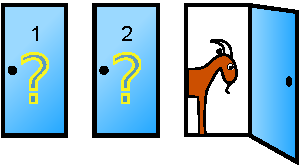
\includegraphics[height=2cm]{img/monty/Monty_open_door}
  \end{center}
\end{frame}


%%% Bibliography

\bibliography{monty,biblio}
\bibliographystyle{apalike}

\end{document}


